%!TEX program = lualatex
\documentclass[12pt, a4paper]{article}
\usepackage[czech]{babel}
\title{The Gevo Times}

%Packages
\usepackage[dvipsnames]{xcolor}


\usepackage[utf8]{inputenc}
\usepackage{amsmath}
\usepackage{amsfonts}
\usepackage{amssymb}

\usepackage[a4paper,includeheadfoot,margin=1cm]{geometry}


\usepackage{multicol}

\usepackage{tikz}
\usetikzlibrary{positioning}

%\usepackage{showframe}


\usepackage{graphicx}

\usepackage{wrapfig}

\usepackage{float}

\usepackage{url}

\usepackage[pdfpagemode=FullScreen, colorlinks=false]{hyperref}

\usepackage{anyfontsize}

\usepackage{emoji}
\usepackage[labelformat=empty]{caption}
\usepackage{qrcode}

%Defining things
\definecolor{gray}{rgb}{0.4,0.4,0.4}

%Header
\usepackage{fancyhdr}
\pagestyle{fancy}


\lhead{
	\footnotesize \thepage.
	}
\chead{
	\textbf{
		{\fontsize{45}{54}\selectfont The GEVO Times}
		}
	}

\rhead{
	\footnotesize Prosinec 2022 %\\[-1\baselineskip] 
	}

\lfoot{

	  }
\cfoot{ \footnotesize
	Veškerý obsah najdete na webových stránkách gevotimes.gevo.cz \\
	Na Facebooku jsme jako The GEVO Times a na Instagramu jako @gevotimes \\
	Grafika a rozvržení: Eric Dusart
	}
\rfoot{\footnotesize

	}
\renewcommand{\headrulewidth}{0pt}
\renewcommand{\footrulewidth}{0.4pt}	% bar on bottom of page

\begin{document}

\sffamily

	\begin{tikzpicture}[remember picture,overlay]
        \node [yshift=0mm] (logo) at (current page.north)
            {\color{gray} \rule{\linewidth}{0pt}};
        \node [below=20mm of logo](first)
            {\color{gray} \rule{\linewidth}{1pt}}
            ;
		\node [below=-2mm of first](second)
		{\color{black} \rule{\linewidth}{3pt}}
		;
		\node [below=-2mm of second](third)
		{\color{gray} \rule{\linewidth}{1pt}}
		;
    \end{tikzpicture}

	\setlength{\columnsep}{30pt}
	\begin{multicols*}{2}
		\setlength{\columnseprule}{1pt}
		\begin{center}\section*{GEVO stánek na veletrhu středních škol}\end{center}
		Schola pragensis je každoroční veletrh středních škol v Praze. Je pořádána pražským magistrátem a koná se v kongresovém centru. Do něj se vždy sjede většina středních škol a snaží se upoutat bezradné deváťáky. Mezi nimi bylo letos i GEVO, ale má to jeden háček. Naše škola není dohledatelná na stránkách Scholy Pragensis. Jediný způsob, jak se dostat k profilu Geva, je přes stažení aplikace, v té už je.

		\noindent Na stánku Geva se během tří dnů konání tohoto veletrhu vystřídalo hned několik studentů a profesorů. Právě těch jsme se ptali, jak si reprezentaci školy užili a co potenciální studenty nejvíce zajímalo.
		\linebreak
		\subsection*{Co jste na místě dělali?}
		Přímo na stánku jsme rozdávali letáky všem, co přišli, a odpovídali jim na otázky o škole. Profesorka Dimmerová nám přímo říkala, ať jim odpovídáme upřímně a studium u nás nijak nepříkrášlujeme.

		\subsection*{Jaká byla nejčastější otázka od dětí?}
		Tak nejčastěji se ptali rodiče a děti se spíš jen vláčeli. Ale nejvíc je zajímalo IB studium. To jsme chválili, protože nám přijde jako super věc. Další časté téma bylo školné, tento dotaz jsme rovnou přesměrovávali na pana ředitele. Zajímala je také výuka angličtiny a třetích jazyků. Angličtinu jsme taky vychvalovali, ti, kdo v prváku přišli a nic neuměli, ve čtvrťáku mluví skvěle. Třetí jazyky jsou taky fajn, hlavně pořádají nejrůznější akce, které jsme rádi zmiňovali.

		\subsection*{Když se někdo ptal čistě na vaši zkušenost, co jste na škole vychvalovali a co hanili?}
		Tak nepříjemností je rozhodně umístění  Jižní Město je na okraji Prahy a hodně lidí to má daleko. V tom je například lepší Sázavská tím, že je v centru. Poté chybějící tělocvična a jídelna, ty existenci na škole znepříjemňují. Tím list negativ končí a můžeme se přesunout k tomu, co nás na škole opravdu baví.

		\noindent Výjimečnost této školy spočívá hlavně v profesorech, jejich přístup a styl učení je něco velmi odlišného od toho, co člověk potká na základní škole.Také pořádáme spoustu školních akcí jako například projektový týden a různé výlety. Důležité nám přišlo zmínit výuku s rodilými mluvčími, protože je velmi efektivní.

		\subsection*{Co uchazeče z pozitiv zaujalo nejvíc?}
		Jakmile jsme zmínili iPady jako školní pomůcky, vždycky se dětem rozzářily oči. Na IB zase slyšeli rodiče. Milý přístup profesorů je něco, co od školy chce každý, a tak rozhodně zaujalo, že GEVO nabízí právě to.
		\vspace*{-1\baselineskip}
		\begin{flushright}
			\footnotesize Jáchym Löwenhöffer
		\end{flushright}
		
		\begin{center}
			\section*{Za východem \emoji{sun} na Sněžku}
		\end{center}
		O projektovém týdnu jsme se vydali na východ slunce na Sněžku s panem profesorem Kejhou. Náš výlet začal ve Vrchlabí, kde jsme si dali pořádný oběd. Z Vrchlabí jsme potom popojeli autobusem do Strážného, odkud jsme vyšli na Dvorskou boudu. S počasím to nevypadalo hezky. Vypadalo to, že bude pořád sněžit. Na Dvorskou boudu jsme přišli za tmy. Další den jsme vyšli ve 4:30 směrem na Luční boudu, kde jsme si dali svačinu. Počasí nám pořád nepřálo, bylo -8°C a sněžilo. Na Sněžku jsme přišli v 7:30, přesně, když má vycházet slunce, ale bohužel vrchol Sněžky byl v mracích. Sestoupili jsme o pár desítek metrů a najednou slunce vykouklo z mraků. Mohli jsme vyfotit hezké fotky východu slunce a já jsem nafilmoval zrychlené video. V 10 hodin jsme došli hladoví do Pece pod Sněžkou a odpočinuli jsme si v restauraci. Poté jsme odjeli zpět do Prahy.

		\begin{flushright}
			\footnotesize Eric Dusart
		\end{flushright}
		\vspace*{-1.5\baselineskip}
		\begin{figure}[H]
			\begin{center}
				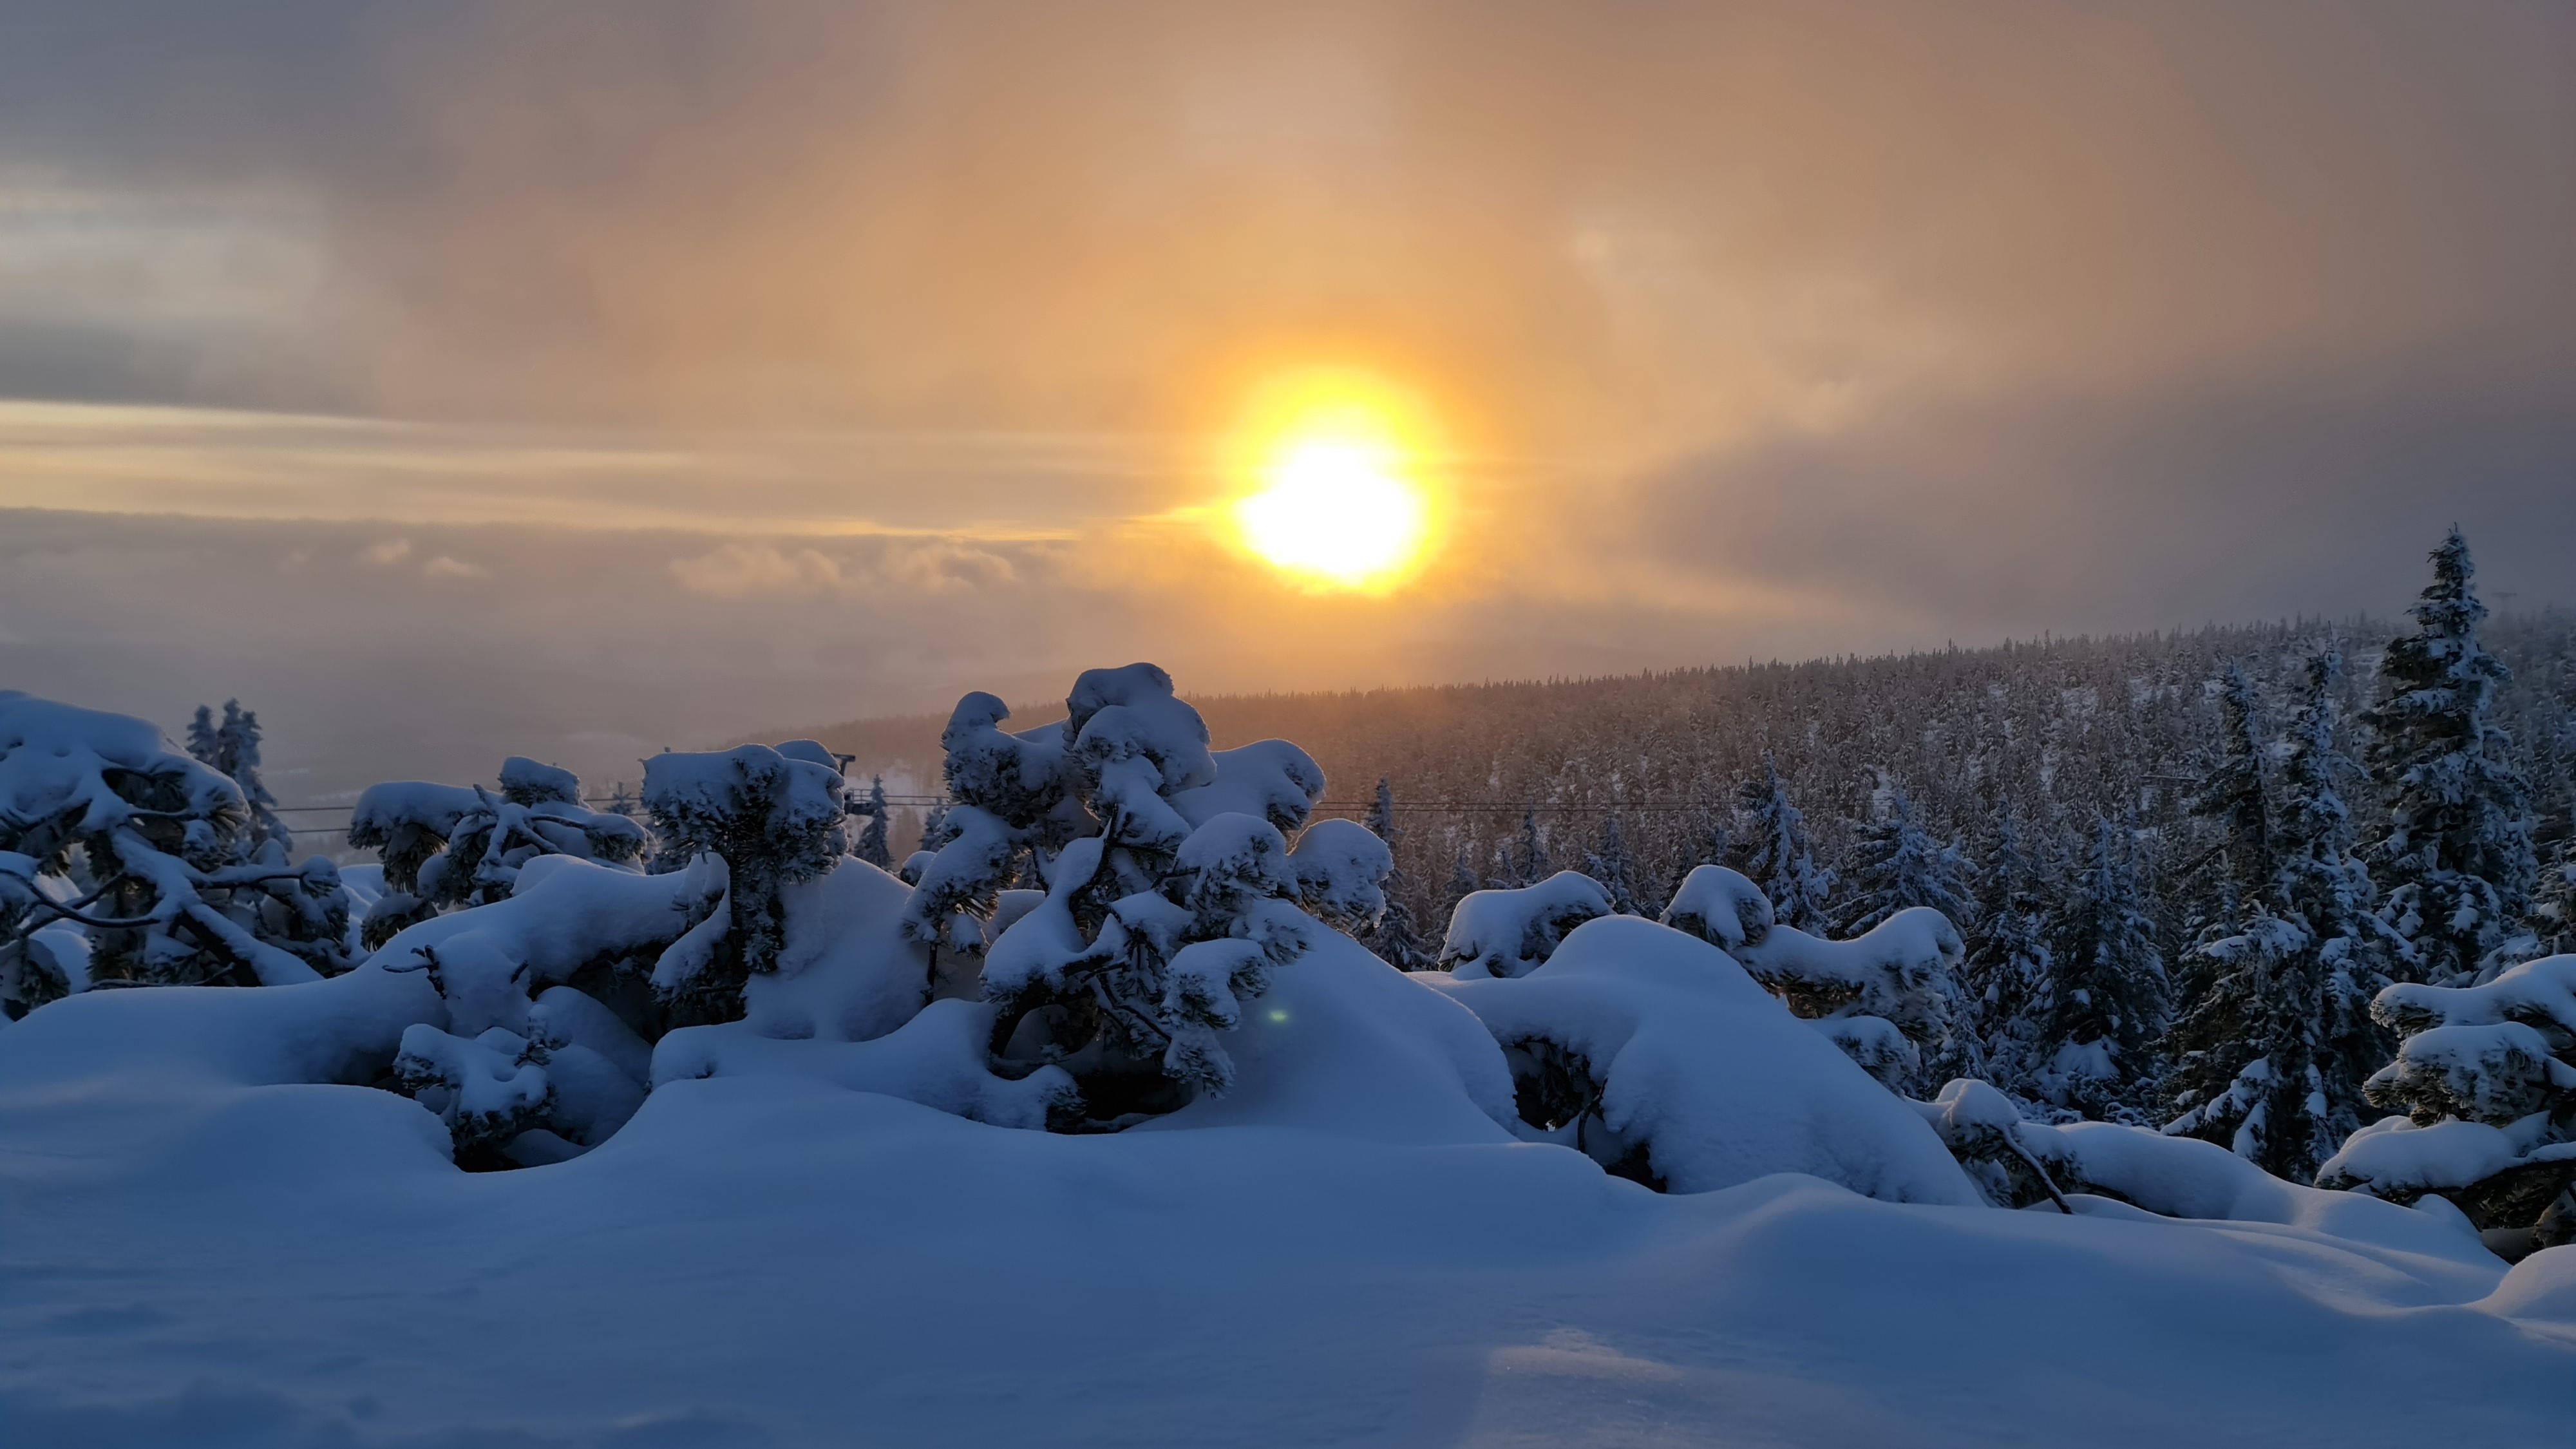
\includegraphics[width=0.28\textwidth]{Snezka4}
				\caption{\footnotesize Východ slunce pod Sněžkou | Fotil: Jakub Šimek}
			\end{center}
		\end{figure}


	\end{multicols*}
	\newpage
	\begin{tikzpicture}[remember picture,overlay]
        \node [yshift=0mm] (logo) at (current page.north)
            {\color{gray} \rule{\linewidth}{0pt}};
        \node [below=20mm of logo](first)
            {\color{gray} \rule{\linewidth}{1pt}}
            ;
		\node [below=-2mm of first](second)
		{\color{black} \rule{\linewidth}{3pt}}
		;
		\node [below=-2mm of second](third)
		{\color{gray} \rule{\linewidth}{1pt}}
		;
    \end{tikzpicture}
	\begin{multicols*}{2}
		\setlength{\columnseprule}{1pt}

		\begin{center}\section*{Fast fashion}\end{center}
		\subsection*{Co je to fast fashion?}
		Fast fashion je způsob masivní výroby oblečení, které je trendy, levné a často i nekvalitní. Problematika fast fashion zahrnuje přílišnou výrobu oblečení v krátkém časovém období, což je velmi neekologické. Navíc se neupotřebí všechno oblečení, které je tímto stylem vyprodukováno. Obchody vytvářejí tlak na jednotlivé skupiny lidí, které ten tlak změní na náhled, který donutí ostatní lidi, aby si zboží koupili a zapadli do davu.

		Dalším problémem fast fashion je špatná kvalita. Materiál je vyrobený levně, a produkty z něj se tím pádem i levně prodávají. Jenže moc dlouho nevydrží a za chvíli si musíte koupit jiný produkt. Proto je třeba zvážit, jestli je lepší koupit si levné levné tričko z polyesteru za dvě stě korun, přičemž za rok si budete muset koupit tři další, anebo si koupit jedno dražší, kvalitní tričko z bavlny za osm set korun, které vydrží celý rok. Nebo stoprocentní vlněnou šálu. Samozřejmě, že bude dražší než polyesterová, ale zase dlouho vydrží. Hlavně levně než kvalitně a ekologicky, na tom je fast fashion hodně postavená.

		\subsection*{Co je to Greenwashing?}
		Greenwashing je situace, kdy organizace nakládá více času a peněz na pojmenování sebe sama šetrný k prostředí než uskutečnění skutečného minimalizování svého dopadu na životní prostředí. Například když nějaký obchod říká, že má 100\% recyklované bundy, ale ve skutečnosti je recyklovaná jedna ze sta.

		\subsection*{Slow fashion}
		Dražší značky, do kterých se vyplatí investovat, protože jejich produkty jsou šetrné k životnímu prostředí a vydrží mnohem déle + vypadají mnohem lépe. V Česku je mnoho značek zaměřených na pomoc životnímu prostředí. Secondhand obchody jsou velmi nápomocné.

		\subsection*{Alternativy}
		Proto tu máme několik návrhů na alternativy. Samozřejmě jednou z už známějších možností je nakupování v  secondhandu, což je podle mě velmi dobrá možnost. Nebo si jednoduše půjčit věci od kamarádů nebo rodiny, co oni už nenosí. Nebo můžete věci taky zdědit. Ano, možná ne vždy nutně najdete to, co se vám líbí, a proto tu máme ještě jednu možnost: swap. Stručně řečeno, měníte oblečení, co už nenosíte, za oblečení jiných lidí, co oni už taky nenosí a vám se líbí. Takhle můžete sehnat věci, co máte rádi, a zároveň omezujete fast fashion. A pokud i tak opravdu chcete nakupovat oblečení v nákupních centrech, tak existuje jedna aplikace – Good on you – co vám řekne, jak moc je daný obchod nebo značka přátelská k přírodě a jak kvalitní jejich výrobky jsou, což se rozhodně hodí.

		Více se dočtete na:
		%\vspace*{-10pt}
		\begin{center}
			\qrcode[hyperlink,height=0.75in]{https://www.businessnewsdaily.com/10946-greenwashing.html}
			\qrcode[hyperlink,height=0.75in]{https://goodonyou.eco}
			\qrcode[hyperlink,height=0.75in]{https://instagram.com/swap_prague?igshid=YmMyMTA2M2Y=}
		\end{center}

		\begin{flushright}
			\footnotesize Karolína Elisabeth Bednářová
		\end{flushright}
		

		


		


		
	\end{multicols*}

	\newpage

	\begin{tikzpicture}[remember picture,overlay]
        \node [yshift=0mm] (logo) at (current page.north)
            {\color{gray} \rule{\linewidth}{0pt}};
        \node [below=20mm of logo](first)
            {\color{gray} \rule{\linewidth}{1pt}}
            ;
		\node [below=-2mm of first](second)
		{\color{black} \rule{\linewidth}{3pt}}
		;
		\node [below=-2mm of second](third)
		{\color{gray} \rule{\linewidth}{1pt}}
		;
    \end{tikzpicture}

	\begin{multicols*}{2}
		\setlength{\columnseprule}{1pt}

		\begin{center}\section*{MIP}\end{center}
		\subsection*{Od Gilgameše po Schrödingera aneb proč číst školní noviny}

		Pokud Vás neodradil název tohoto článku, tak upřímně
		gratuluji a za vaši odvahu vám nyní dlužím vysvětlení
		podstaty několika vět, které hodlám napsat. Rozhodl
		jsem se naše skvělé noviny obohatit článkem, který
		bude do jisté míry informovat o~událostech domácích či
		světových, aktuálních či již dávno minulých, zkrátka o
		různých zajímavostech, které vám mohou rozšířit vaše
		obzory a pomoci třeba i se školou. A toto mám v plánu
		dělat dokonce pravidelně v každém vydání GEVO
		Times. Článek bych pojmenoval „MIP” (Měsíční informační
		přehled).

		A jak jinak začít první díl MIPu vydávaného v~prosinci 
		než jakousi vánoční tematikou.

		Vánoce se slaví prakticky všude, ovšem v každém koutě
		světa oslavují tuto tradici trochu jinak a jindy. Nemusí
		se jednat pouze o státy spojené s~křesťanstvím.
		Například v Číně nosí dárky Tun Čche Lao-žen, na Havaji
		Kanakaloka a v Itálii Babbo Natálie. Kde to ale všechno
		začalo? Po pravdě to nikdo neví přesně, s největší
		pravděpodobností je ale tato tradice rozdávání dárků
		spojena se svatým Mikulášem. Ten se narodil roku 270
		n.l. v dnešním Turecku. Jeho rodiče byli hodně bohatí,
		ovšem zemřeli, když byl Mikuláš ještě mladý, a tedy
		nestačil ještě zcela ovládnout finanční gramotnosti. A jelikož
		to byl dobrý člověk, celý svůj nemalý majetek rozdal
		potřebným lidem. Za důkaz toho, že byl tak štědrý,
		považujeme příběhy, které se z té doby o Mikulášovi
		dochovaly. Nejznámější z nich je příběh O vdovci a jeho
		třech dcerách. V dobách dávno minulých se dívky
		provdávaly jen pod podmínkou, že měly věno, tedy
		majetek, kterým by mohly přispět do budoucí společné
		domácnosti. Tento vdovec však neměl žádné peníze a
		proto se jeho dcery nemohly vdát. Nezbývalo mu tedy
		nic jiného než dcery prodat do otroctví. Tomu ovšem
		zabránil náš Mikuláš, který se o tom dozvěděl, v noci se
		potichu dostal na vdovcovu střechu a do komína jim
		hodil tři měšce peněz. Vdovec tak nemusel dcery
		prodat a ony se mohly v poklidu vdát.

		Mikuláš poté vykonal další štědré skutky, za které byl
		jmenován biskupem z Myry. Zemřel 6. prosince roku
		345 nebo 352 n.l. Povědomí o něm rozšířily francouzské
		jeptišky, které nemocným v klášterech 6. prosince
		večer rozdávaly dárky. Marodící ráno byli šťastní a
		zvědaví, kdo jim je nadělil. Jeptišky vždy odpověděly, že
		to byl asi svatý Mikuláš\dots

		Doufám, že se vám tohle povídání líbilo a bylo pro vás
		alespoň trochu informativní. Přeji vám všem hezké
		Vánoce a za měsíc se těším u dalšího dílu MIP.
		\begin{flushright}
			\footnotesize Jiří Průša
		\end{flushright}

		\vspace*{-2\baselineskip}
		\begin{center}\section*{Nadpis}\end{center}
		


	\end{multicols*}

	\newpage
	\begin{tikzpicture}[remember picture,overlay]
        \node [yshift=0mm] (logo) at (current page.north)
            {\color{gray} \rule{\linewidth}{0pt}};
        \node [below=20mm of logo](first)
            {\color{gray} \rule{\linewidth}{1pt}}
            ;
		\node [below=-2mm of first](second)
		{\color{black} \rule{\linewidth}{3pt}}
		;
		\node [below=-2mm of second](third)
		{\color{gray} \rule{\linewidth}{1pt}}
		;
    \end{tikzpicture}
	\vspace*{-1.5\baselineskip}
	\begin{center}\section*{Výstup projektu o fast fashion}\end{center}
	\vspace*{-2\baselineskip}
	\begin{figure}[H]
		\centering
		\includegraphics[width=0.9\textwidth]{ko}
	 \end{figure}

\end{document}
